\documentclass[10pt]{article}
\usepackage[letterpaper,margin=0.72in,headheight=15pt]{geometry}
\usepackage[T1]{fontenc}
\usepackage[utf8]{inputenc}
\usepackage{lmodern}
\usepackage{microtype}
\usepackage{parskip}
\usepackage{enumitem}
\usepackage{booktabs}
\usepackage{tabularx}
\usepackage{longtable}
\usepackage{array}
\usepackage{xcolor}
\usepackage[most]{tcolorbox}
\usepackage{fancyhdr}
\usepackage{hyperref}
\usepackage{amsmath,amssymb}
\usepackage{listings}
\usepackage{tikz}
\usetikzlibrary{arrows.meta,positioning,shapes.geometric,fit}
\usepackage{needspace}
\usepackage{multicol}
\usepackage{lastpage}
\usepackage{titlesec}

\definecolor{navy}{HTML}{17324D}
\definecolor{bluegray}{HTML}{43657D}
\definecolor{lightblue}{HTML}{EAF2F8}
\definecolor{lightgray}{HTML}{F3F5F7}
\definecolor{linegray}{HTML}{C9D1D9}
\definecolor{darkgray}{HTML}{4A5561}
\definecolor{accent}{HTML}{8E3B46}

\hypersetup{colorlinks=true,linkcolor=navy,urlcolor=bluegray,citecolor=navy,pdfborder={0 0 0}}
\setlist[itemize]{leftmargin=1.4em,itemsep=2pt,topsep=4pt}
\setlist[enumerate]{leftmargin=1.6em,itemsep=2pt,topsep=4pt}
\renewcommand{\arraystretch}{1.22}
\setlength{\tabcolsep}{4pt}
\newcolumntype{Y}{>{\raggedright\arraybackslash}X}
\newcolumntype{C}[1]{>{\centering\arraybackslash}p{#1}}
\newcolumntype{L}[1]{>{\raggedright\arraybackslash}p{#1}}
\pagestyle{fancy}
\fancyhf{}
\lhead{Application Security Engineering}
\rhead{Code Review Handbook}
\cfoot{\thepage\ of \pageref{LastPage}}
\renewcommand{\headrulewidth}{0.4pt}
\titleformat{\section}{\Large\bfseries\color{navy}}{\thesection}{0.65em}{}
\titleformat{\subsection}{\large\bfseries\color{bluegray}}{\thesubsection}{0.55em}{}
\titleformat{\subsubsection}{\normalsize\bfseries\color{darkgray}}{\thesubsubsection}{0.5em}{}
\titlespacing*{\section}{0pt}{1.4em}{0.55em}
\titlespacing*{\subsection}{0pt}{1.0em}{0.35em}

\newcommand{\checkbox}{\ensuremath{\square}}
\newcommand{\fieldline}[1]{\textbf{#1}\hspace{0.5em}\leaders\hbox{\rule[0.4ex]{0.6em}{0.35pt}\hspace{0.25em}}\hfill\kern0pt}
\newcommand{\workarea}[1]{\par\smallskip\noindent\begin{tcolorbox}[height=#1,colback=white,colframe=linegray,boxrule=0.5pt,arc=0pt,left=2pt,right=2pt,top=2pt,bottom=2pt]\mbox{}\end{tcolorbox}\par}
\newtcolorbox{keybox}[1]{colback=lightblue,colframe=bluegray,title=\textbf{#1},fonttitle=\bfseries,boxrule=0.7pt,arc=2pt,left=6pt,right=6pt,top=5pt,bottom=5pt}
\newtcolorbox{cautionbox}[1]{colback=lightgray,colframe=accent,title=\textbf{#1},fonttitle=\bfseries,boxrule=0.7pt,arc=2pt,left=6pt,right=6pt,top=5pt,bottom=5pt}
\newtcolorbox{worksheetbox}[1]{colback=white,colframe=linegray,title=\textbf{#1},fonttitle=\bfseries,coltitle=navy,boxrule=0.6pt,arc=1pt,left=6pt,right=6pt,top=5pt,bottom=5pt}
\lstset{basicstyle=\ttfamily\small,columns=fullflexible,breaklines=true,frame=single,framerule=0.4pt,rulecolor=\color{linegray},backgroundcolor=\color{lightgray},showstringspaces=false,tabsize=2,keywordstyle=\bfseries}
\setcounter{tocdepth}{2}

\title{\textbf{Code Audit Strategy Catalog}\\\large Application Security Engineering Handout}
\author{}
\date{}

\begin{document}
\maketitle
\thispagestyle{empty}
\begin{keybox}{Purpose}
Practitioner catalog for selecting macro-level code-audit strategies and combining them across a review.
\end{keybox}
\vfill
\noindent\textbf{Use note.} This handout is a practitioner aid for authorized software security assessment. It emphasizes evidence, traceability, and disciplined review rather than a single rigid methodology.
\newpage
\tableofcontents
\newpage

\section{Strategy vs. Technique}
A \textbf{strategy} is the macro-level route through the assessment: where the reviewer starts, what path is followed, which abstraction is targeted, and what evidence marks completion. A \textbf{technique} is a localized analytical method used while executing that route. Mature assessments combine strategies and switch between them as system understanding improves.

\section{Code Navigation Model}
\subsection{External Flow Sensitivity}
External flow describes how aggressively a reviewer follows execution and data between functions or modules. Four practical modes are useful:
\begin{itemize}
\item \textbf{Control-flow insensitive, data-flow insensitive:} review the current function/module largely in isolation; record external questions rather than immediately following them.
\item \textbf{Control-flow sensitive:} follow calls that affect the selected execution path.
\item \textbf{Data-flow sensitive:} follow propagation of selected data and ignore unrelated calls.
\item \textbf{Control- and data-flow sensitive:} reason about both reachability and values across calls. This provides richer path context but creates more mental context switching.
\end{itemize}
The choice is a complexity-management decision, not a quality grade. A reviewer can intentionally ignore external flow during module review and still perform detailed internal flow analysis inside each function.

\subsection{Tracing Direction}
\begin{center}
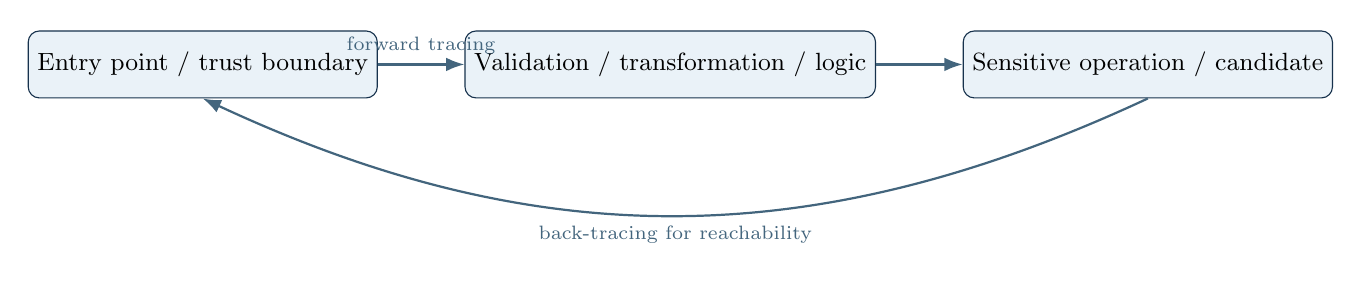
\begin{tikzpicture}[node distance=11mm, box/.style={draw=navy,rounded corners,minimum width=3.4cm,minimum height=0.85cm,align=center,fill=lightblue,font=\small}, arr/.style={-Latex,thick,color=bluegray}]
\node[box] (entry) {Entry point / trust boundary};
\node[box,right=of entry] (logic) {Validation / transformation / logic};
\node[box,right=of logic] (sink) {Sensitive operation / candidate};
\draw[arr] (entry)--node[above,font=\scriptsize]{forward tracing}(logic);
\draw[arr] (logic)--(sink);
\draw[arr] (sink.south) to[bend left=25] node[below,font=\scriptsize]{back-tracing for reachability} (entry.south);
\end{tikzpicture}
\end{center}

\textbf{Forward tracing} commonly starts at entry points, trust boundaries, module beginnings, or key algorithms and asks what can happen as execution/data moves inward. \textbf{Back-tracing} commonly starts at a candidate sink, crash, or automated finding and asks whether attacker influence can reach it. Back-tracing reduces initial path count, but its coverage is constrained by candidate selection and it is weaker for pure logic/design flaws.
\clearpage

\section{Strategy Taxonomy}
\begin{center}
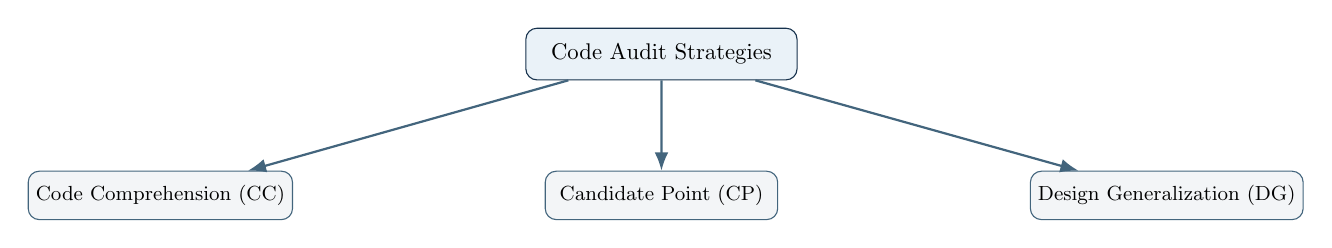
\begin{tikzpicture}[scale=0.82,transform shape,node distance=8mm, root/.style={draw=navy,rounded corners,fill=lightblue,minimum width=4.2cm,minimum height=.8cm,align=center}, child/.style={draw=bluegray,rounded corners,fill=lightgray,minimum width=3.6cm,minimum height=.75cm,align=center,font=\small}, arr/.style={-Latex,thick,color=bluegray}]
\node[root] (r) {Code Audit Strategies};
\node[child,below left=14mm and 36mm of r] (cc) {Code Comprehension (CC)};
\node[child,below=14mm of r] (cp) {Candidate Point (CP)};
\node[child,below right=14mm and 36mm of r] (dg) {Design Generalization (DG)};
\draw[arr] (r)--(cc); \draw[arr] (r)--(cp); \draw[arr] (r)--(dg);
\end{tikzpicture}
\end{center}

\par\smallskip\noindent\begin{tabularx}{\linewidth}{@{}L{0.24\linewidth}L{0.30\linewidth}Y@{}}
\toprule
Family & Core idea & Typical value \\
\midrule
Code Comprehension & Read implementation directly to find vulnerabilities while learning how the system works & Rich understanding; can expose subtle implementation and logic issues \\
Candidate Point & Generate potential issues first, then validate their relevance and reachability in code & Fast prioritization and broad coverage of known weakness patterns \\
Design Generalization & Infer or validate higher-level behavior and security design from implementation & Medium- to high-level logic, policy, and architectural defects \\
\bottomrule
\end{tabularx}

\section{Standard Strategy Card}
Each catalog entry uses the same decision fields so strategies can be selected deliberately. Difficulty and speed are qualitative because they vary with reviewer experience and application familiarity.
\clearpage

\section{Code Comprehension Strategies}

\Needspace{12\baselineskip}
\subsection{CC1 -- Trace Malicious Input}
\par\smallskip\noindent\begin{tabularx}{\linewidth}{@{}L{0.25\linewidth}Y@{}}
\toprule
Family & Code Comprehension \\
Objective & Follow attacker-influenced data from an entry point toward security-sensitive behavior. \\
Recommended use & Early or middle review when entry points are known and path-level reasoning is valuable. \\
Starting point & Data entry point / trust boundary \\
Ending point & Validated vulnerability, safe termination, or bounded analysis goal \\
Tracing direction / sensitivity & Forward; usually control-flow and data-flow sensitive; High for the selected path \\
Typical abstraction & Basic implementation through implementation logic \\
Relative difficulty / speed & Hard / Very slow \\
Comprehension benefit & High \\
Strengths & Naturally concentrates on security-relevant code; can expose subtle validation and trust-boundary defects. \\
Blind spots / failure modes & Path expansion can become extreme; interprocedural context switching causes fatigue; easy to skip callees late in a long session. \\
Suggested companion techniques & Internal flow analysis; subsystem analysis; test cases \\
Evidence to capture & Entry point, propagated data, validation/transformation points, sinks, discarded branches, unresolved callees \\
Exit criteria & Chosen path reaches a meaningful sink/termination or remaining branches are explicitly deferred. \\
Example workflow & Choose an API parameter controlled by a remote caller; trace transformations and checks until the data reaches a file, query, command, allocator, or authorization decision. \\
\bottomrule
\end{tabularx}

\Needspace{12\baselineskip}
\subsection{CC2 -- Analyze a Module}
\par\smallskip\noindent\begin{tabularx}{\linewidth}{@{}L{0.25\linewidth}Y@{}}
\toprule
Family & Code Comprehension \\
Objective & Read a cohesive source file or module line by line while minimizing external jumps. \\
Recommended use & Useful early for learning project idioms and in cohesive modules where local context is rich. \\
Starting point & Start of source file / module \\
Ending point & End of source file / module \\
Tracing direction / sensitivity & Forward; externally control-flow insensitive and data-flow insensitive; Local context high; external context intentionally limited \\
Typical abstraction & Basic implementation through design \\
Relative difficulty / speed & Very hard / Slow \\
Comprehension benefit & Very high \\
Strengths & Builds familiarity with language, wrappers, conventions, and developer patterns; reduces mental context switching. \\
Blind spots / failure modes & Mentally taxing; can consume time on code that later proves low risk; requires disciplined candidate notes. \\
Suggested companion techniques & Rereading; internal flow analysis; application-specific candidate points \\
Evidence to capture & Functions reviewed, local assumptions, suspicious calls, candidate points, cross-module questions \\
Exit criteria & Module is completely reviewed at the chosen depth and deferred external questions are recorded. \\
Example workflow & Review a shared utility module without following every call. Record unsafe-looking contracts and revisit them later through candidate or dependency analysis. \\
\bottomrule
\end{tabularx}

\Needspace{12\baselineskip}
\subsection{CC3 -- Analyze an Algorithm}
\par\smallskip\noindent\begin{tabularx}{\linewidth}{@{}L{0.25\linewidth}Y@{}}
\toprule
Family & Code Comprehension \\
Objective & Examine a security-relevant algorithm as one bounded unit. \\
Recommended use & Middle review after enough design understanding exists to identify critical algorithms. \\
Starting point & First implementation element of the selected algorithm \\
Ending point & End of the algorithm / defined algorithm boundary \\
Tracing direction / sensitivity & Forward; external flow usually limited unless context is required; High inside the algorithm \\
Typical abstraction & Basic implementation through design \\
Relative difficulty / speed & Very hard / Slow \\
Comprehension benefit & Very high \\
Strengths & Strong focus prevents irrelevant wandering; suitable for subtle logic, state, and boundary defects. \\
Blind spots / failure modes & Can lack caller/callee context; difficult algorithms impose high cognitive load. \\
Suggested companion techniques & Desk-checking; test cases; internal flow analysis; peer review \\
Evidence to capture & Algorithm contract, invariants, state transitions, edge cases, assumptions, candidate findings \\
Exit criteria & Algorithm behavior and security invariants are explained with no unresolved critical branch. \\
Example workflow & Analyze an authorization decision algorithm, derive its allowed state transitions, and desk-check unusual combinations of identity, resource, and policy state. \\
\bottomrule
\end{tabularx}

\Needspace{12\baselineskip}
\subsection{CC4 -- Analyze a Class or Object}
\par\smallskip\noindent\begin{tabularx}{\linewidth}{@{}L{0.25\linewidth}Y@{}}
\toprule
Family & Code Comprehension \\
Objective & Review an object as a stateful abstraction: interface, lifecycle, invariants, and methods. \\
Recommended use & Object-oriented code where behavior is distributed across methods and state members. \\
Starting point & Class / object interface and implementation \\
Ending point & Complete object lifecycle and relevant consumers \\
Tracing direction / sensitivity & Primarily forward with selective call tracing; Moderate to high \\
Typical abstraction & Basic implementation through design \\
Relative difficulty / speed & Very hard / Slow \\
Comprehension benefit & Very high \\
Strengths & Keeps related state and methods together; effective for invariant and lifecycle defects. \\
Blind spots / failure modes & Inheritance, callbacks, and framework behavior can hide external state changes or alternate dispatch. \\
Suggested companion techniques & Rereading; internal flow; dependency analysis; hypothesis testing \\
Evidence to capture & Public methods, privileged methods, state fields, invariants, lifecycle transitions, callers requiring follow-up \\
Exit criteria & All security-relevant methods and state transitions have been reviewed at the selected depth. \\
Example workflow & Map a session object from construction through authentication, privilege changes, invalidation, and destruction; test whether any method violates lifecycle invariants. \\
\bottomrule
\end{tabularx}

\Needspace{12\baselineskip}
\subsection{CC5 -- Trace Dynamic-Test Hits}
\par\smallskip\noindent\begin{tabularx}{\linewidth}{@{}L{0.25\linewidth}Y@{}}
\toprule
Family & Code Comprehension \\
Objective & Start from observed runtime behavior and trace into implementation to explain the root condition. \\
Recommended use & When dynamic testing, fuzzing, IAST, or manual runtime probing has produced a reproducible anomaly. \\
Starting point & Reproducible runtime hit / crash / anomaly \\
Ending point & Root cause and attacker-influence explanation \\
Tracing direction / sensitivity & From runtime symptom into code; direction may alternate; High near the observed path \\
Typical abstraction & Implementation through implementation logic \\
Relative difficulty / speed & Moderate to hard / Medium \\
Comprehension benefit & High \\
Strengths & Provides concrete evidence and a known trigger; narrows initial search space. \\
Blind spots / failure modes & Observed symptom can be secondary; may over-focus on one crash while missing related patterns. \\
Suggested companion techniques & Debugger tracing; internal flow; back-tracing; application-specific candidate search \\
Evidence to capture & Trigger, stack/trace, path, state, root cause, related-pattern search \\
Exit criteria & Root cause is mapped to reachable attacker influence and sibling instances are considered. \\
Example workflow & Reproduce a parser crash, map the failing instruction to source, identify the length/state relationship, then search for other uses of the same parsing idiom. \\
\bottomrule
\end{tabularx}
\clearpage

\section{Candidate Point Strategies}

\Needspace{12\baselineskip}
\subsection{CP1 -- General Candidate Point Approach}
\par\smallskip\noindent\begin{tabularx}{\linewidth}{@{}L{0.25\linewidth}Y@{}}
\toprule
Family & Candidate Point \\
Objective & Begin at a security-relevant operation and determine whether attacker-controlled state can reach it unsafely. \\
Recommended use & Broadly useful when dangerous sinks or operations can be enumerated. \\
Starting point & Candidate operation / sink \\
Ending point & Entry point, trusted constraint, or evidence that candidate is not exploitable \\
Tracing direction / sensitivity & Backward tracing; sensitivity chosen as needed; Focused \\
Typical abstraction & Basic implementation through implementation logic \\
Relative difficulty / speed & Moderate / Fast to medium \\
Comprehension benefit & Medium \\
Strengths & Limits the number of paths compared with forward tracing; efficient for known weakness classes. \\
Blind spots / failure modes & Coverage is only as good as candidate selection; logic flaws may not map to obvious sinks. \\
Suggested companion techniques & Constraint establishment; internal flow; test cases \\
Evidence to capture & Candidate origin, backward path, attacker influence, constraints, disposition \\
Exit criteria & Candidate is validated, rejected with evidence, or escalated for deeper analysis. \\
Example workflow & Start at a dynamic SQL execution API and trace each parameter backward to its sources, transformations, validation, and trust boundary. \\
\bottomrule
\end{tabularx}

\Needspace{12\baselineskip}
\subsection{CP2 -- SAST-Assisted Candidate Points}
\par\smallskip\noindent\begin{tabularx}{\linewidth}{@{}L{0.25\linewidth}Y@{}}
\toprule
Family & Candidate Point \\
Objective & Use automated source analysis to produce candidate locations, then perform human validation. \\
Recommended use & Early for broad pattern discovery and throughout the review as a supplement to manual analysis. \\
Starting point & Tool finding / candidate list \\
Ending point & Manual disposition with reachability and impact evidence \\
Tracing direction / sensitivity & Usually backward from reported sink/source pair; Varies by tool and rule \\
Typical abstraction & Basic implementation through implementation logic \\
Relative difficulty / speed & Easy to moderate / Fast \\
Comprehension benefit & Low to medium \\
Strengths & Scales candidate discovery and supports repeatability across large codebases. \\
Blind spots / failure modes & False positives, modeled-library gaps, path truncation, and rule coverage limits; tool severity is not exploitability. \\
Suggested companion techniques & Back-tracing; test cases; module analysis \\
Evidence to capture & Rule, location, tool path, manually verified path, environmental assumptions, disposition \\
Exit criteria & Every selected high-value candidate has a documented manual disposition. \\
Example workflow & Prioritize findings on dangerous file/path operations, then manually verify source controllability, canonicalization, authorization, and reachable runtime configuration. \\
\bottomrule
\end{tabularx}

\Needspace{12\baselineskip}
\subsection{CP3 -- Lexical Candidate Points}
\par\smallskip\noindent\begin{tabularx}{\linewidth}{@{}L{0.25\linewidth}Y@{}}
\toprule
Family & Candidate Point \\
Objective & Locate risky APIs, constructs, or project idioms with text / structural search and validate each hit. \\
Recommended use & Early review for known APIs and after learning project-specific wrappers. \\
Starting point & Search pattern / symbol / construct \\
Ending point & Candidate disposition \\
Tracing direction / sensitivity & Backward or local analysis from each hit; Low initially; increases during validation \\
Typical abstraction & Basic implementation \\
Relative difficulty / speed & Easy / Very fast discovery; validation varies \\
Comprehension benefit & Low to medium \\
Strengths & Simple, transparent, and easy to customize; excellent for repeated unsafe idioms. \\
Blind spots / failure modes & Misses semantic equivalents, aliases, wrappers, and logic vulnerabilities; noisy patterns can waste time. \\
Suggested companion techniques & Module analysis; application-specific candidate points; dependency analysis \\
Evidence to capture & Search definition, result set, exclusions, validation notes, pattern refinements \\
Exit criteria & Search space and each selected hit are documented; unresolved classes are recorded. \\
Example workflow & Search for direct process-execution APIs, then expand the pattern to local wrappers discovered during module review. \\
\bottomrule
\end{tabularx}

\Needspace{12\baselineskip}
\subsection{CP4 -- Binary Candidate Points}
\par\smallskip\noindent\begin{tabularx}{\linewidth}{@{}L{0.25\linewidth}Y@{}}
\toprule
Family & Candidate Point \\
Objective & Identify suspicious operations or instruction patterns in compiled code and back-trace reachability and control. \\
Recommended use & Binary-only or mixed reviews where source is unavailable or incomplete. \\
Starting point & Binary call site / instruction sequence / imported dangerous API \\
Ending point & Reachable input source or evidence of safe constraint \\
Tracing direction / sensitivity & Backward through control/data dependencies; Selective \\
Typical abstraction & Basic implementation through implementation logic \\
Relative difficulty / speed & Hard / Slow to medium \\
Comprehension benefit & Medium \\
Strengths & Provides a structured starting point when source is unavailable; can reveal behavior omitted from documentation. \\
Blind spots / failure modes & Optimization, stripped symbols, indirect calls, and compiler transformations complicate reasoning. \\
Suggested companion techniques & Debugger analysis; hypothesis testing; runtime tracing \\
Evidence to capture & Address/symbol, call context, xrefs, path constraints, runtime confirmation \\
Exit criteria & Candidate is tied to a reachable path and its security consequence is understood. \\
Example workflow & Find calls to a risky memory-copy routine in a stripped binary, trace callers, then confirm suspicious length propagation dynamically. \\
\bottomrule
\end{tabularx}

\Needspace{12\baselineskip}
\subsection{CP5 -- Dynamic / Black-Box Candidate Points}
\par\smallskip\noindent\begin{tabularx}{\linewidth}{@{}L{0.25\linewidth}Y@{}}
\toprule
Family & Candidate Point \\
Objective & Turn crashes, exceptions, malformed output, or behavioral anomalies into implementation candidates. \\
Recommended use & When external testing produces repeatable signals but the root condition is not known. \\
Starting point & Observed anomaly \\
Ending point & Root condition and reachable attacker-controlled trigger \\
Tracing direction / sensitivity & Back-tracing from symptom with dynamic evidence; High around the observed execution \\
Typical abstraction & Implementation through implementation logic \\
Relative difficulty / speed & Moderate / Medium \\
Comprehension benefit & Medium to high \\
Strengths & Starts with concrete behavior; good bridge between dynamic testing and code review. \\
Blind spots / failure modes & Symptom can occur far from the defect; absence of anomalies says little about untested logic. \\
Suggested companion techniques & Debugger tracing; application-specific candidate search; desk-checking \\
Evidence to capture & Trigger, environment, crash/trace, candidate location, root cause, related instances \\
Exit criteria & Root cause is explained and sibling conditions have been considered. \\
Example workflow & Use a fuzz-generated exception to locate a parser boundary failure, then inspect nearby parser helpers for the same assumption. \\
\bottomrule
\end{tabularx}

\Needspace{12\baselineskip}
\subsection{CP6 -- Application-Specific Candidate Points}
\par\smallskip\noindent\begin{tabularx}{\linewidth}{@{}L{0.25\linewidth}Y@{}}
\toprule
Family & Candidate Point \\
Objective & Generalize a risky implementation idiom discovered in the target and search for related instances. \\
Recommended use & Middle or late review after developer patterns, wrappers, and local abstractions are understood. \\
Starting point & Validated target-specific risky pattern \\
Ending point & All relevant sibling instances triaged \\
Tracing direction / sensitivity & Pattern discovery followed by local/backward validation; Varies \\
Typical abstraction & Basic implementation through design \\
Relative difficulty / speed & Moderate / Fast once pattern is known \\
Comprehension benefit & High \\
Strengths & Converts learned application context into high-yield broad coverage; catches custom wrappers generic tools miss. \\
Blind spots / failure modes & Poorly generalized patterns create noise or miss semantically similar variants. \\
Suggested companion techniques & Module analysis; lexical search; SAST custom rules; subsystem analysis \\
Evidence to capture & Canonical example, generalized pattern, search method, result set, dispositions \\
Exit criteria & Pattern definition is stable and relevant instances are triaged or explicitly deferred. \\
Example workflow & After finding a custom authorization helper that trusts a cached flag, search for all calls and related helpers that use the same flag as an access decision. \\
\bottomrule
\end{tabularx}
\clearpage

\section{Design Generalization Strategies}

\Needspace{12\baselineskip}
\subsection{DG1 -- Model the System}
\par\smallskip\noindent\begin{tabularx}{\linewidth}{@{}L{0.25\linewidth}Y@{}}
\toprule
Family & Design Generalization \\
Objective & Reverse-engineer architecture and security behavior from implementation evidence. \\
Recommended use & Bottom-up reviews and poorly documented subsystems where high-level design must be reconstructed. \\
Starting point & Implementation evidence from selected subsystem \\
Ending point & Useful working model validated against code \\
Tracing direction / sensitivity & Varies; iterative abstraction from code; High at selected areas \\
Typical abstraction & Implementation logic through architectural \\
Relative difficulty / speed & Very hard / Very slow \\
Comprehension benefit & Very high \\
Strengths & Can reveal undocumented trust boundaries and design flaws; produces durable understanding. \\
Blind spots / failure modes & High effort; model can be distorted by early assumptions; easy to over-model low-value details. \\
Suggested companion techniques & Hypothesis testing; derive purpose/function; module analysis \\
Evidence to capture & Components, relationships, trust levels, assumptions, confidence, contradicting evidence \\
Exit criteria & Model explains security-relevant behavior well enough to guide the next review strategy. \\
Example workflow & Reconstruct an identity subsystem from entry handlers, token parsing, policy checks, and session storage, then compare inferred trust boundaries with observed callers. \\
\bottomrule
\end{tabularx}

\Needspace{12\baselineskip}
\subsection{DG2 -- Hypothesis Testing}
\par\smallskip\noindent\begin{tabularx}{\linewidth}{@{}L{0.25\linewidth}Y@{}}
\toprule
Family & Design Generalization \\
Objective & Form a claim about what a code element represents and test it against implementation evidence. \\
Recommended use & Medium to large systems where no reviewer can hold the entire design in working memory. \\
Starting point & Code element plus an explicit hypothesis \\
Ending point & Supported, revised, or rejected hypothesis \\
Tracing direction / sensitivity & Varies; Evidence-driven \\
Typical abstraction & Implementation logic through architectural \\
Relative difficulty / speed & Hard / Medium \\
Comprehension benefit & Very high \\
Strengths & Faster than fully modeling everything; forces assumptions to become testable statements. \\
Blind spots / failure modes & Poor assumptions can misdirect later review; confirmation bias is a major failure mode. \\
Suggested companion techniques & Peer review; module analysis; internal flow; system modeling \\
Evidence to capture & Hypothesis, supporting evidence, conflicting evidence, confidence, next test \\
Exit criteria & Hypothesis is accepted with bounded confidence, rejected, or replaced by a better hypothesis. \\
Example workflow & Hypothesize that a cache is authoritative for authorization; inspect population, invalidation, and consumer paths for evidence supporting or contradicting that claim. \\
\bottomrule
\end{tabularx}

\Needspace{12\baselineskip}
\subsection{DG3 -- Derive Purpose and Function}
\par\smallskip\noindent\begin{tabularx}{\linewidth}{@{}L{0.25\linewidth}Y@{}}
\toprule
Family & Design Generalization \\
Objective & Infer the security purpose, trust level, privileges, interfaces, and larger-system role of key implementation elements. \\
Recommended use & When implementation is understood locally but its place in the security model is unclear. \\
Starting point & Security-relevant code element \\
Ending point & Documented abstraction and its security relationships \\
Tracing direction / sensitivity & Varies; High \\
Typical abstraction & Implementation logic through architectural \\
Relative difficulty / speed & Hard / Medium \\
Comprehension benefit & Very high \\
Strengths & Focuses modeling effort on known security-relevant areas and exposes architectural assumptions. \\
Blind spots / failure modes & Mentally taxing; wrong inferred purpose can contaminate later analysis. \\
Suggested companion techniques & Hypothesis testing; trust-boundary mapping; design conformity \\
Evidence to capture & Purpose summary, trust levels, privileges, interfaces, consumers, confidence \\
Exit criteria & The element can be placed coherently in the security model with explicit evidence and uncertainty. \\
Example workflow & Summarize a token-validation component: what trust it establishes, which claims it owns, what callers rely on, and what privileges follow. \\
\bottomrule
\end{tabularx}

\Needspace{12\baselineskip}
\subsection{DG4 -- Design Conformity Check}
\par\smallskip\noindent\begin{tabularx}{\linewidth}{@{}L{0.25\linewidth}Y@{}}
\toprule
Family & Design Generalization \\
Objective & Compare implementation behavior with intended design or policy and analyze security consequences of deviations. \\
Recommended use & Later review when design intent and actual behavior are both sufficiently understood. \\
Starting point & Module / component with stated expected behavior \\
Ending point & End of selected behavior plus impact analysis of deviations \\
Tracing direction / sensitivity & Usually forward; control-flow and data-flow sensitive where required; High \\
Typical abstraction & Implementation logic through design \\
Relative difficulty / speed & Moderate / Medium \\
Comprehension benefit & Medium \\
Strengths & Good balance of implementation and design reasoning; bounded when the specification is clear. \\
Blind spots / failure modes & Quality depends on the design's accuracy; a policy deviation is not automatically a security vulnerability. \\
Suggested companion techniques & Internal flow; test cases; derive purpose/function \\
Evidence to capture & Expected behavior, actual behavior, gray areas, deviations, affected paths, security impact \\
Exit criteria & Meaningful deviations are dispositioned as benign policy differences or security-relevant findings. \\
Example workflow & Compare authorization requirements with every implementation branch, especially undefined cases and error paths, then trace any variance to concrete security impact. \\
\bottomrule
\end{tabularx}

\section{Strategy Selection Matrix}
\scriptsize
\begin{longtable}{@{}L{0.07\linewidth}L{0.12\linewidth}L{0.10\linewidth}L{0.10\linewidth}L{0.10\linewidth}L{0.11\linewidth}L{0.11\linewidth}L{0.12\linewidth}@{}}
\toprule
ID & Review stage & Source need & Runtime need & App knowledge & Main strength & Main limitation & Typical automation role \\
\midrule
\endfirsthead
\toprule
ID & Review stage & Source need & Runtime need & App knowledge & Main strength & Main limitation & Typical automation role \\
\midrule
\endhead
CC1 & Early--mid & High & Optional & Low--mid & Security-relevant path focus & Path explosion & Navigation / data-flow assistance \\
CC2 & Early--mid & High & No & Low & Learns project idioms & High cognitive cost & Search / cross-reference support \\
CC3 & Mid--late & High & Optional & Mid & Deep algorithm reasoning & Requires correct target selection & Test generation / navigation aid \\
CC4 & Mid & High & Optional & Mid & Lifecycle and invariant focus & Indirect dispatch complexity & Class hierarchy / call graph support \\
CC5 & Any after runtime hit & Helpful & High & Low--mid & Concrete trigger & Symptom may be secondary & DAST / fuzz / IAST generation \\
CP1 & Any & Usually high & Optional & Low & Efficient reachability check & Candidate-selection bias & Candidate discovery \\
CP2 & Early--continuous & High & No & Low & Scalable breadth & False positives / model gaps & Core mechanism \\
CP3 & Early--continuous & High & No & Low & Transparent broad search & Lexical blind spots & Core mechanism \\
CP4 & Binary reviews & No & Helpful & Mid--high & Works without source & Reverse-engineering complexity & Pattern/xref discovery \\
CP5 & Any after runtime hit & Optional & High & Low & Evidence-driven starting point & Limited to observed behavior & Core runtime discovery \\
CP6 & Mid--late & High & Optional & High & Target-specific high yield & Pattern generalization risk & Custom searches / custom rules \\
DG1 & Mid--late & High or binary & Helpful & Growing & Architectural understanding & Slow and assumption-heavy & Diagram extraction aid only \\
DG2 & Mid--late & High or binary & Optional & Mid & Makes assumptions testable & Confirmation bias & Evidence collection aid \\
DG3 & Mid--late & High or binary & Optional & Mid--high & Reconstructs security purpose & Mentally taxing & Navigation / summarization aid \\
DG4 & Late / whenever intent known & High & Helpful & High & Design vs. implementation reasoning & Bad specification can mislead & Difference discovery aid \\
\bottomrule
\end{longtable}
\normalsize

\section{Strategy Composition Patterns}
\par\smallskip\noindent\begin{tabularx}{\linewidth}{@{}L{0.34\linewidth}Y@{}}
\toprule
Composition & Why it works \\
\midrule
Lexical search $\rightarrow$ candidate validation $\rightarrow$ module analysis & Uses cheap discovery for breadth, then deepens only where evidence justifies it. \\
Dynamic hit $\rightarrow$ back-trace $\rightarrow$ algorithm analysis & Converts observable behavior into root-cause reasoning and precise edge-case analysis. \\
Module analysis $\rightarrow$ application-specific candidate search & Learns local wrappers and idioms first, then scales that knowledge across the codebase. \\
Bottom-up comprehension $\rightarrow$ system modeling $\rightarrow$ design conformity & Builds reliable design knowledge from implementation before judging policy/specification deviations. \\
SAST candidate $\rightarrow$ constraint establishment $\rightarrow$ targeted test case & Separates tool suspicion from actual reachability and exploitability. \\
\bottomrule
\end{tabularx}
\clearpage

\section{One-Page Strategy Decision Aid}
\begin{enumerate}
\item \textbf{Do you have a concrete runtime symptom?} Start with CC5 or CP5, then back-trace and analyze the responsible algorithm/module.
\item \textbf{Do you have a dangerous sink or automated candidate?} Use CP1/CP2/CP3/CP4, then validate attacker influence and constraints.
\item \textbf{Are you still learning the codebase?} Use CC2/CC4 on cohesive implementation units; record application-specific idioms.
\item \textbf{Do you know a critical algorithm?} Use CC3 with desk-checking and boundary test cases.
\item \textbf{Is design documentation weak?} Use DG1/DG2/DG3 to build the security model from code.
\item \textbf{Is intended behavior known?} Use DG4 to compare policy/specification with actual implementation, but assess security impact separately from mere nonconformity.
\item \textbf{At every switch:} record why the next strategy has higher expected value than continuing the current one.
\end{enumerate}

\begin{keybox}{Selection Rule}
There is no universal best strategy. Select the strategy whose starting information you actually possess, whose blind spots are acceptable for the current review stage, and whose expected evidence advances the assessment's stated objective.
\end{keybox}
\end{document}
